\chapter{Garment Depth Map Clustering}
\label{garment_clustering}

This chapter explains in detail the garment depth map clustering stage that our algorithm performs to the garment data previously segmented. In this stage, the depth image data is preprocessed using the segmentation results from the previous stage to remove all depth data not related to the garment. Then, it applies a Watershed transform algorithm to find the different similar-height regions, that will be analyzed in the last stage to select the most suitable manipulation points to unfold the garment. \juansays{(Referenciar figura)}

\begin{figure}[thpb]
    \centering
    
\includegraphics[width=0.7
    \textwidth]{figures/placeholder2.png}
    \caption{\comment{(Block diagram for Garment Depth Map Clustering chapter)}}
    \label{fig:garment_clustering_blocks}
\end{figure}

\section{Depth Image Preprocessing}
\label{depth_image_preprocessing}

The raw depth image data obtained from the robot sensor requires some treatment before it can be processed in the next step (section \ref{garment_clustering_watershed}). This step takes the garment mask calculated in the previous stage, and applies it to the depth image of the garment. The objective is to discard the information related to the table. 

As the next step will treat the depth data as a greyscale image, the remaining garment depth data is normalized to the 8-bit range of a typical greyscale image. By normalizing the data we ensure that we are using the maximum resolution available (256 grey levels) to represent all the depth variability in the depth image. This helps the next step to find similar-height regions more accurately.

Figure \ref{fig:depth_map_preprocessing} \comment{[...]}

\begin{figure}[thpb]
    \centering
    
\includegraphics[width=0.7
    \textwidth]{figures/placeholder2.png}
    \caption{\comment{(Figure representing this preprocessing step)}}
    \label{fig:depth_map_preprocessing}
\end{figure}


\section{Similar-Height Region Clustering}
\label{garment_clustering_watershed}

Once the garment depth data is separated from the table depth data and normalized in the previous step, similar-height regions must be identified and labeled.

Grouping points according to a common feature such as height is a clustering problem, and several clustering methods and alternatives were described in section \ref{architecture:depth_map_clustering}. Some of the superpixel segmentation algorithms were tested during the development of this work, but finally a Watershed \reftodo algorithm was selected to perform the clustering. This algorithm is faster than other superpixel approaches, \comment{[...]}

The Watershed transform is a segmentation algorithm that considers a greyscale image as a topological surface where high intensity pixels correspond to peaks and hills, and low intensity pixels are equivalent to valleys. The algorithm fills the surface pouring water at each isolated valley. As the water level rises, the water from different sources will start to merge. To prevent them from merging, the algorithm constructs barriers at the merging regions, and continues this process of adding water and building barriers until all the peaks have been flooded. The resulting barriers are the segmentation result, where each region enclosed correspond to a segmented item. Figure \ref{fig:watershed_example} shows an example of applying the Watershed algorithm to segment coins.

\begin{figure}[thpb]
    \centering
    
\includegraphics[width=0.7
    \textwidth]{figures/placeholder2.png}
    \caption{\comment{(Here it would be great to add a figure of the example, such as opencv's coins)}}
    \label{fig:watershed_example}
\end{figure}

A denoising process is performed before applying the Watershed transform, which is the actual clustering process. We use a Total Variation filter \reftodo{\comment{[chambolle]}} to produce a smoother image while maintaining the edges sharp. The Total Variation filter works by minimizing the integral of the norm of the image gradient. As a result of this filter, piecewise-constant images (``cartoon-like'' images) are obtained.

The Watershed segmentation algorithm is then applied to the depth image of the garment to locate the different parts that are overlapping each other. These regions are related to folded parts, that rest on top of other parts of the garment. 
%
As, in practice, flooding using local minima as markers \juansays{(Revisar "markers")} leads to over-segmentation, an enhanced version\footnote{\url{http://scikit-image.org/docs/dev/auto_examples/segmentation/plot_marked_watershed.html}} of this algorithm  allows the user to specify other criteria for selecting the seed points. The gradient of the greyscale depth-image is computed, and regions where the gradient has a low value are selected as these seed points. These regions correspond to homogeneous and continous regions, which are good candidates to be used as markers.

The different garment regions obtained with Watershed were labeled and used as input for the next step. Figure \ref{fig:watershed_labels} shows the result of this process.

\begin{figure}[thpb]
    \centering
    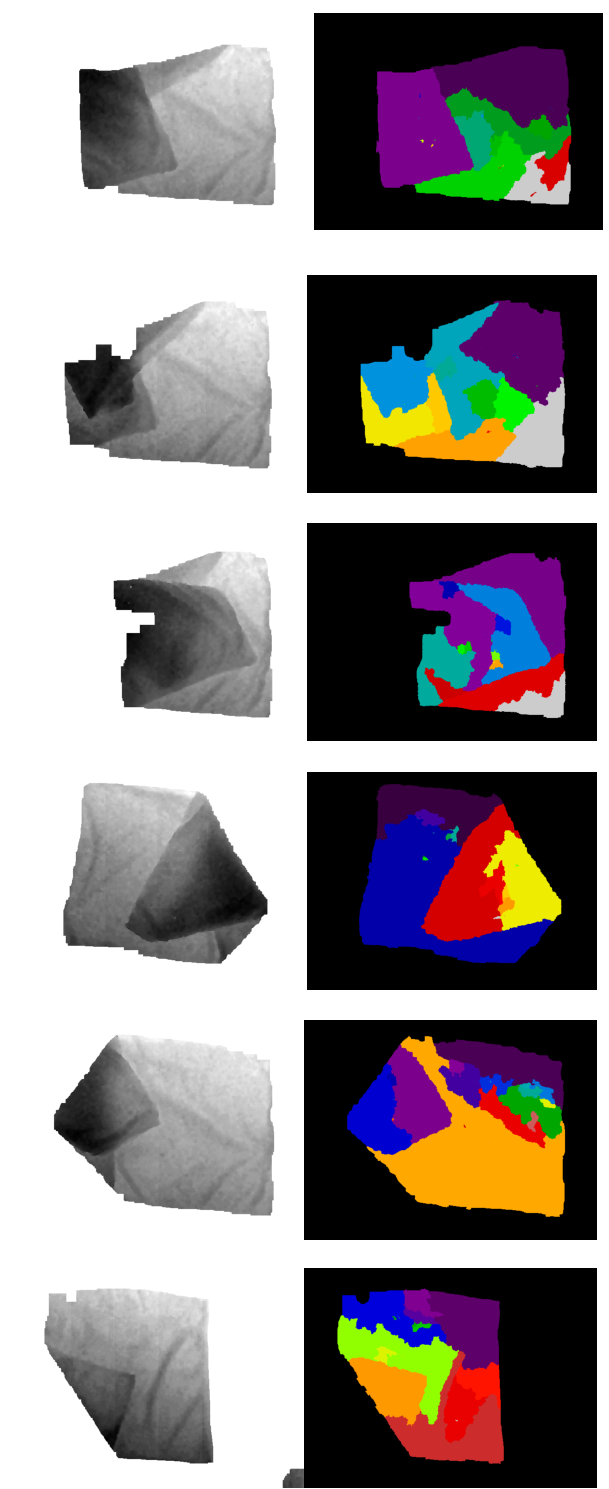
\includegraphics[width=0.58\textwidth]{figures/colour_garment.pdf}
    \caption{On the left side, the grayscale images are shown. The grey level is related to the height of the point as detected by the RGB-D sensor. On the right side, the labeled image returned by watershed algorithm is presented, where each color represents a region of similar height.}
    \label{fig:watershed_labels}
\end{figure}
